\documentclass[11pt]{article}
\usepackage[utf8]{inputenc}
\usepackage{graphicx}
\date{}
\usepackage{titlesec}
\begin{document}
\title{\line(1,0){250} \\ \huge{\textbf{2019-2020 Bahar Yarıyılı \\ BLM2512 Veri Yapıları ve Algoritmalar 3. Ödevi}} \\\line(1,0){250}}
\author{\textsc{Mesut Şafak Bilici} \\ 17011086}
\maketitle
\section{1 Algoritma ve Fonksiyonlar}
\textit{\large{1.1 Makrolar}}\\
\hspace*{1cm} Kod boyunca kullanılacak dizilerin boyutu için makrolar belirlenmiştir. Bu makrolar aşağıdaki gibidir:
\begin{itemize}
	\item \textbf{MAX\_FILE\_NAME:} Text'in okunması için açılacak dosyanın 			   isminin maksimum uzunluğunu belirler.
	\item \textbf{MAX\_TEXT\_LENGTH:} Okunan text'in maximum karakter sayısını
		   belirler. Test sırasında arttırılması için kod esnek yazılmıştır.
	\item \textbf{MAX\_SUBSTRING\_LENGTH:} Text'İn içinde olan sub-text'in
		   maksimum karakter sayısıdır. Bu sub-text daha sonra 				 			   değiştirilecektir. Bu makro aynı zamanda subtext'in değiştirileceği
		   string için de karakter sayısı olarak belirlenmiştir.
\end{itemize}
\textit{\large{1.2 Fonksiyonlar ve Algoritmik Açıklamaları}}\\
\hspace*{1cm} Kodda yapılan algoritmik işlemlerin hepsi fonksiyonlar üzerinden yürütlmüştür. Main fonksiyonu bir sonraki bölümde açıklanmak üzere kullanılan fonksiyonlar ve açıklamaları aşağıdaki gibidir:
\begin{itemize}
	\item \textbf{int} \textsf{abs\_sub(char,char):} İki char'ın ASCII
	değerini alıp farkının mutlak değerini döndüren fonksiyon. Bu fonksiyon
	Boyer-Moore Algoritması'nın non-case sensitivite seçeneğinde kullanılıp
	o kısımda daha detaylı açıklanacaktır.
	
	\item \textbf{int} \textsf{shiftTable(char*,int*,int,int):} Boyer-Moore
	algoritmasında ne kadar 'skip' yapacağımız için kullanılmaktadır. Bir
	offset/başlangıç ASCII değeri kullanılarak yapılsa da algoritmamızda
	iki farklı case seçeneği bulunduğu için tüm ASCII değerlerini alacak 
	şekilde hazırlanmıştır Shift Table. İlk parametresinde bulunması 
	istenilen sub\-string'i, ikinci parametresinde main içinde dinamik olarak
	tanımlanan Shift Table dizisini, üçüncü parametresinde istendiği zaman 
	kullanılması için-esneklik için yazılan offset değeri, dördüncü 
	parametresinde ise Shift Table'ımızın boyunu veriyoruz. Sub'string'in
	içinde olmayan her karakter için Shift Table'ın her cell'i -1 değerini
	alırken içinde olan karakterler de index değerini alıyor. 
	
	\item \textbf{int} \textsf{BoyerMoore(char*,char*,int*,int*):} Boyer 
	Moore algoritmasının case sensitivite halidir. Kullanıcı case sensitivite 
	arama yapacağı zaman kullanılacak fonksiyondur. Bu fonksiyon ilk 
	parametresinde text char array'ini, ikinci parametresinde
	substring char array'ini, üçüncü parametresinde öncesinde belirlenen
	Shift Table integer array'ini almıştır. Dördüncü parametrenin yaptığı iş
	fonsiyon her çalıştırıldığında ve her -1'den farklı değer döndürdüğünde
	1 arttırılmaktır, yani fonksiyon her çalıştığında ve her çalıştığında 
	yeni bir belirlenen substring'i bulduğun-\\da 1 arttırılıyor. Bu yapılan
	işlem maşn fonksiyonu içinde neden sürekli fonksiyonu çağırmamız 
	gerektiğinin açıklaması yapıldığında daha anlamlı olacaktır. While 
	döngüsünden çıkıldığı an ve j sıfır değerinden küçük olduğu an 
	substring'i text içinde buluğumuzu anlıyoruz, ve sonrasında bu 
	substring'in text içindeki index konumunu döndürüyoruz.
	
	\item \textbf{int} \textsf{BoyerMoore\_noncase(char*,char*,int*,int*):} 
	Tüm parametreleri yu-\\karda açıklanan case sensitivite Boyer Moore
	algoritması olmakla beraber yaptığı iş de kısmi olarak aynıdır. Fakat 
	kaynak kod incelendiği zaman fark edilecektir ki bu sefer while içindeki
	koşullar biraz farklıdır. Burada öncesinde tanımladığımız
	\textit{abs\_sub} fonksiyonunu kullanacağız. While içindeki $j>=$ 
	koşulu aynıdır fakat $substring[j] == buffer[i+j]$ yerine, \\ $abs			 	\_sub(substring[j], buffer[i+j]) == 0 \\ || \\abs\_sub(substring[j],buffer[i		    +j])==32)$,
	\\
	koşulları kullanılmıştır. Görüldüğü üzere yukarıda verilen mantıksal     		ifadenin ilk elemanı aslında case sensitivite Boyer Moore'daki \\
    $substring[j] == buffer[i+j]$ \\
    ifadesi ile birebir aynı. İkinci mantıksal ifadede belirtilen şey, eğer
    substring'in içinde geldiğimiz bir karakter text'in içindeki karakterin
    küçük harf versiyonuysa veya tam tersi büyük harf versiyonuysa bu ikisini
    aynı kabul et. Anlamsal olarak aynı olan fakat birisi büyük harf ve
    diğer küçük harf olan iki karakterin ASCII tablosundaki değerlerinin 
    mutlad değer farkı her zaman 32'ye eşittir. Örnek: $A=65$, $a=97$ için 
    $$|A - a| == |a - A| == 32$$
    
    \item \textbf{void} \textsf{replace(char*,char*,char*,int):}
    Substring bulunduktan sonra kullanıcının istediği string ile değiştirmek 
    için kullanılan fonksiyon. İlk parametre olarak dosyadan okunan text'i,
    ikinci parametre olarak bulunan substring'i, üçüncü parametre olarak 
    substring'in yerine yazmak istediğimiz string'i, dördüncü parametre 
    olarak dosyadan okunan text'in içindeki substring'in başlangıç konumunu
    - indexini alıyor. Replace işlemi için toplamda 3 farklı durum 
    değerlendirildi:
    \begin{enumerate}
    	\item Substring'in uzunluğunun replace string'in uzunluğuna eşit
    	olması durumu. Bu durumda iki stringin aynı index'leri sadece 
    	değiştirilecektir.
    	\item Substring'in uzunuluğunun replace string'in uzunluğundan
    	büyük olması durumu. Bu durumda, substring'in replaced string 
    	uzunlu-ğuna kadar replaced stringi atarız. Daha sonra geride    				kalanları substring'in uzunluğu ve replaced string'in uzunluğu farkı  		kadar sola taşırız. Örnek:\\ substring= "find", replaced string= 				"get", strlen(substring) = 4, strlen(replaced string) = 3 ,
    	strlen(substring) - strlen(replaced string) = 1:
    	\begin{enumerate}
    	    \item find this
    		\item getd this $\rightarrow$ boşluk karakteri 1 sola
    		\item get $\; \;$this $\rightarrow$ t karakteri 1 sola
    		\item get tthis $\rightarrow$ h karakteri 1 sola
    		\item get thhis $\rightarrow$ i karakteri 1 sola
    		\item get thiis $\rightarrow$ s karakteri 1 sola
    		\item get thiss $\rightarrow$ bundan sonra null var ise, son s 
    		karakteri yerine null gelir, yoksa eğer bu şekilde model devam
    		eder en son null için aynısı yapılır.
    	\end{enumerate}
    	\item Replace string'in uzunluğunun substring'in uzunluğundan büyük 
    	olma durumu. Bu durumda ilk atama işlemi yerine kaydırma işlemi 
    	yapmamız gerekmekte. Bunu yapmazsak eğer veri kaybı yaşayabiliriz.
    	Text string'inin son karakterinden, yani null, başlayarak replaced
    	string'in uzunluğu ve substring'in uzunluğu farkı sağa kaydırma 
    	yapacağız. Bu kaydırmadan sonra artık atama işlemimizi yapabiliriz.
    	Örnek: \\
    	substring = "pass", replaced string = "passs", strlen(substring) = 4,
    	strlen(replaced string) = 5:
    	\\ Not: Görselleştirme anlaşılsın diye harf büyüklükleri aynı 
    	seçilmek üzere pass için passs kelimesi tercih edilmiştir.
    	\begin{enumerate}
    		\item pass this $\rightarrow$ s karakteri 1 sağa 
    		\item pass thiss $\rightarrow$ i karakteri 1 sağa
    		\item pass thiis $\rightarrow$ h karakteri 1 sağa
    		\item pass thhis $\rightarrow$ t karakteri 1 sağa
    		\item pass tthis $\rightarrow$ boşluk karakteri 1 sağa
    		\item pass $\;$this $\rightarrow$ atama işlemini başlat
    		\item passs this
    	\end{enumerate}
    \end{enumerate}
\end{itemize}
\textit{\large{1.3 Main}}\\
\hspace*{1cm} Bu kısımda Main fonksiyonu içinde yukarıda belirtilen fonksiyonların nasıl kullanıldığı belirtilmekle beraber main fonksiyonunun içinde neler yapıldığı anlatılacaktır.\\
İlk olarak bazı array tanımlamaları gözükmektedir. Bu arraylar sırasıyla,
\begin{itemize}
	\item \textbf{char} \textsf{filename:} Açılacak olan dosyanın ismini
	kullanıcıdan alırken girdiyi bu array'e alıyoruz. Statik olarak açıldı.
	\item \textbf{char*} \textsf{buffer:} Dosyanın içindeki text bilgisini
	bu array'in üstüne yazıyoruz. Array dinamik olarak açılmıştır.
	Daha sonra kullanıcı bu array içinde substring arayacaktır, ve burada
	substring'i değiştirecektir.
	\item \textbf{char*} \textsf{substring:} Kullanıcı buffer array'inin 
	içindeki text'te bir kelime veya cümle bulmak isteyecektir. Bulmak 
	istediği kelime veya cümleyi klavyeden girdi olarak verecektir. 
	Bu girdiyi substring isimli array'de tutuyoruz. Dinamik olarak açıldı.
	\item \textbf{char*} \textsf{replaced:} Kullanıcı substring'i bulduktan
	sonra bu substring'i değiştirecektir. Ne ile değiştirmek istediğini
	klavyeden girdi olarak verecektir. Bu substring'in yerine geçecek olan
	string replaced isimli array'de saklanmaktadır.
	\item \textbf{int*} \textsf{table:} Shift table'ı main içinde dinamik
	olarak açıyoruz. Fonksiyon içinde veri girdisi yapılıyor.
\end{itemize}
Daha sonrasıda ise bazı değişken tanımlamaları gözükmektedir,
\begin{itemize}
	\item \textbf{int} \textsf{case\_ctrl:} Kullanıcının non-case sensitive
	mi yoksa case sensitivite arama yapacağının kontrolünü yapacak
	değişken.
	\item \textbf{int} \textsf{found:} Her yeni sub-string bulunduğunda 
	sayısını gösterecek değşiken.
	\item \textbf{int} \textsf{index:} Her yeni sub-string bulunduğunda 
	text içindeki index'ini gösterecek değşiken.
\end{itemize}
Bu tanımlamalardan sonra içinde text'in olduğu dosyayı açtık ve $fread$ fonksiyonu ile buffer array'ine veriyi yazdık. Daha sonra kullanıcıdan case sensitivite mi yoksa değil mi, sub-string ne, ne ile değiştirilsin bilgileri istenir. Eğer kullanıcı $case\_ctrl$ değişkenini 0 olarak seçerse $BoyerMoore\_noncase()$ fonksiyonu , değilse $BoyerMoore()$ fonksiyonu çalışır. Her iki durumda da $shiftTable()$ fonksiyonu çalıştırılır ve shift table oluşturulur. Daha sonra yukarıdaki arama yapan iki fonksiyonumuzdan teki, case durumuna göre, çağrılır ve bir index döndürür. Bu index, -1 değerinde ise herhangi bir substring bulamamıştır ve bundan sonra da bulamayacaktır. Bu sebepten dolayı aşağıdaki while döngüsüne girmeden devam eder kod. Eğer ki, -1 yerine substring'in olası bir index değerini döndürürse
arama fonksiyonu, while döngüsüne girilir ve başka substring var mı araması yapılır, yenisini buldukçta while içinde bu substring replaced stringi ile değiştirilir. En son bir substring kalmadığında -1 döndürür ve kod devam eder, yeni text'i dosyaya tekrardan yazar.\\  
\textit{\large{1.4 Çalışma Süresi}}\\
\hspace*{1cm} Çalışma süresi saniye cinsinden hesaplanmıştır. Kütüphane olarak time.h kütüphanesi kullanılıp, bu zaman, \\
\hspace*{2cm}- clock\_t t;\\
\hspace*{2cm}- t = clock();\\
\hspace*{3cm} $\vdots$ \\
\hspace*{2cm}- t= clock()-t;\\
\hspace*{2cm}- double time\_taken = ((double)t)/CLOCKS\_PER\_SEC;\\
şeklinde hesaplanmıştır. 
\pagebreak
\section{2 İstenilen Örnekler}
\textit{\large{2.1.1 Örnek}}\\
\hspace*{1cm} \textbf{Find:} algorithm \\
\hspace*{1cm} \textbf{Replace:} method \\
\hspace*{1cm} \textbf{Option:} non case sensitivite \\
\hspace*{1cm} \textbf{Text:} The Boyer-Moore Algorithm is considered the most
efficient string matching algorithm. \\
\hspace*{1cm} \textbf{Output:}
\begin{figure}[h!]
\centering
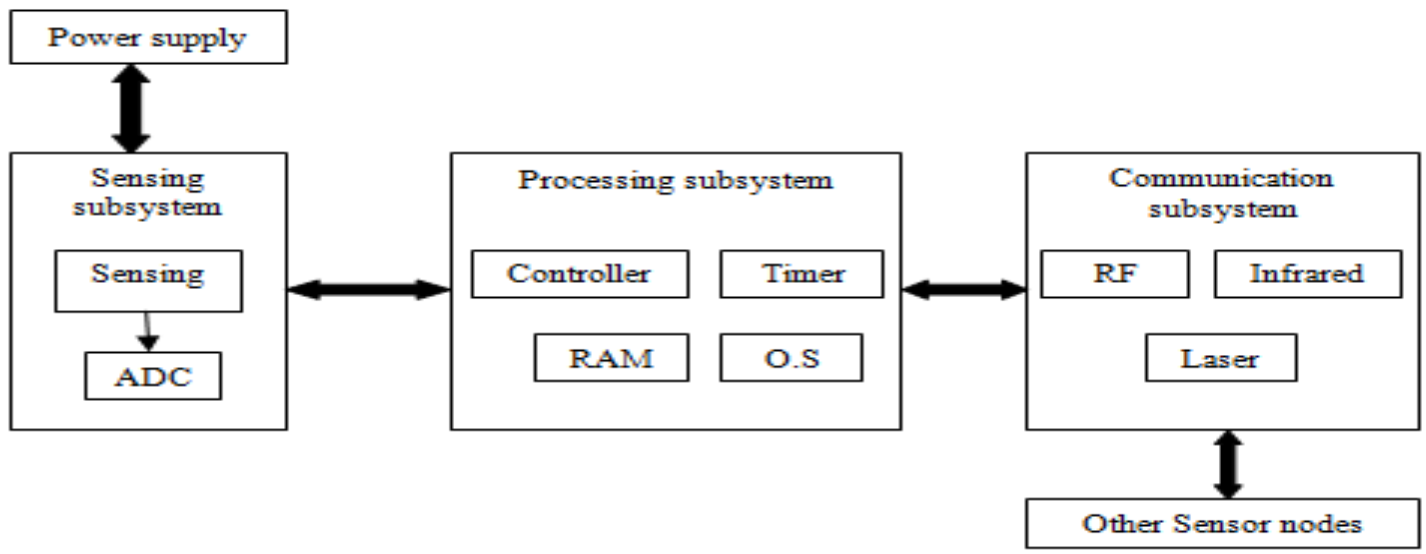
\includegraphics[width=130mm,scale=0.5]{2.png}
\caption{Örnek 1 Non-case Sensitivite}
\label{fig:istenilen}
\end{figure}
\\
\textit{\large{2.1.2 Örnek}}\\
\hspace*{1cm} \textbf{Find:} algorithm \\
\hspace*{1cm} \textbf{Replace:} method \\
\hspace*{1cm} \textbf{Option:} case sensitivite \\
\hspace*{1cm} \textbf{Text:} The Boyer-Moore Algorithm is considered the most efficient string matching algorithm. \\
\hspace*{1cm} \textbf{Output:}
\begin{figure}[h!]
\centering
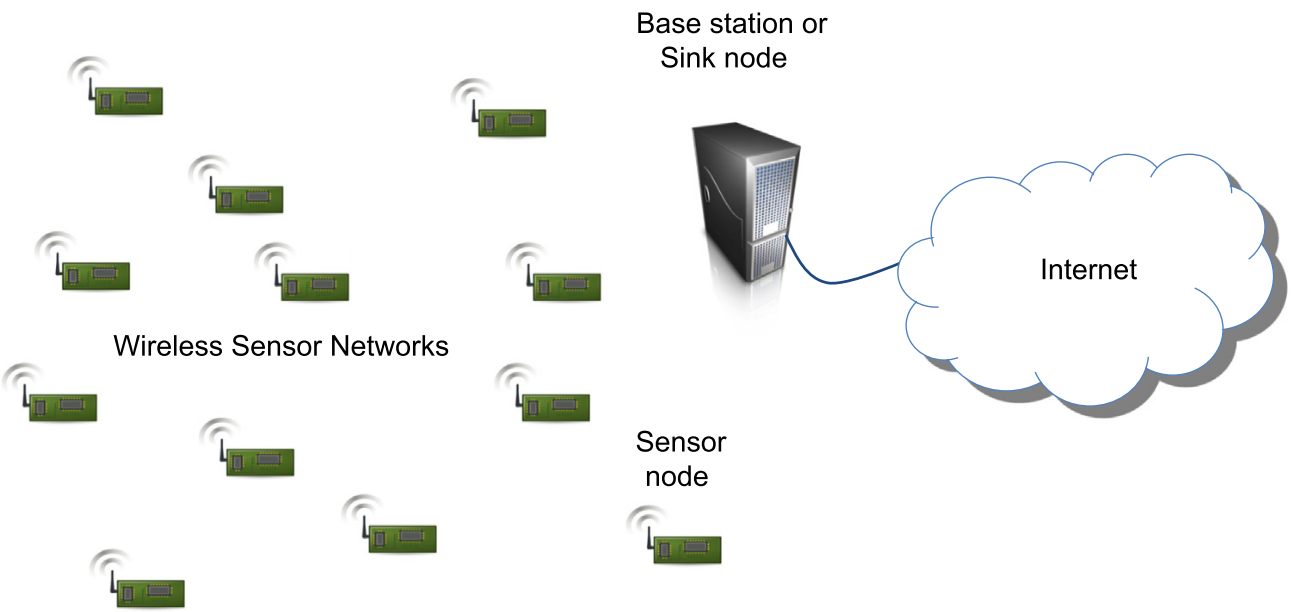
\includegraphics[width=130mm,scale=0.5]{1.png}
\caption{Örnek 1 Case Sensitivite}
\label{fig:istenilen2}
\end{figure}
\pagebreak
\\
\textit{\large{2.2 Örnek}}\\
\hspace*{1cm} \textbf{Find:} went to \\
\hspace*{1cm} \textbf{Replace:} visited \\
\hspace*{1cm} \textbf{Option:} non case sensitivite \\
\hspace*{1cm} \textbf{Text:} Wayne went to Wales to watch walruses. \\
\hspace*{1cm} \textbf{Output:}
\begin{figure}[h!]
\centering

\includegraphics[width=130mm,scale=0.5]{3.png}
\caption{Örnek 2 Non-case Sensitivite}
\label{fig:istenilen3}
\end{figure}\\
\pagebreak
\section{3 Performans}
\hspace*{1cm} Aşağıda göreceğiniz dataframe; yazılan programın farklı text boyutlarında, bu text üzerinde farklı uzunluklardaki ve farklı sayılardaki substring'lerin ve replaced string'lerin değiştirilmesine bağlı, saniye bilgilerini taşımaktadır. Bu veri implemente edilmesi istenen programın defalarca farklı parametreler ile çalıştırılarak elde edilmiştir.
\begin{figure}[h!]
\centering
\includegraphics[width=110mm,scale=0.5]{csv.png}
\caption{Saniyeye bağlı performans verisi}
\label{fig:csv}
\end{figure}\\
Aşağıda ise bu performansı daha iyi yorumlayabilmek için 3 boyutlu öklidyen uzayda görselleştirilmesi yapılmıştır. 
\begin{figure}[h!]
\centering
\includegraphics[width=125mm,scale=0.5]{Figure_1.png}
\caption{Text size 124}
\label{fig:124}
\end{figure}\\
\begin{figure}[h!]
\centering
\includegraphics[width=125mm,scale=0.5]{Figure_2.png}
\caption{Text size 221}
\label{fig:221}
\end{figure}\\
\begin{figure}[h!]
\centering
\includegraphics[width=125mm,scale=0.5]{Figure_3.png}
\caption{Text size 405}
\label{fig:405}
\end{figure}\\
\begin{figure}[t]
\includegraphics[width=125mm,scale=0.5]{Figure_4.png}
\caption{Text size 112}
\label{fig:112}
\end{figure}\\
\end{document}

